\documentclass[12pt]{article}
\usepackage[utf8]{inputenc}
\usepackage[spanish,es-lcroman, es-tabla]{babel}
\usepackage[autostyle,spanish=mexican]{csquotes}
\usepackage{amsmath}
\usepackage{amssymb}
\usepackage{nccmath}
\numberwithin{equation}{section}
\usepackage{amsthm}
\usepackage{graphicx}
\usepackage{epstopdf}
\DeclareGraphicsExtensions{.pdf,.png,.jpg,.eps}
\usepackage{color}
\usepackage{float}
\usepackage{multicol}
\usepackage{enumerate}
\usepackage[shortlabels]{enumitem}
\usepackage{anyfontsize}
\usepackage{anysize}
\usepackage{array}
\usepackage{multirow}
\usepackage{enumitem}
\usepackage{cancel}
\usepackage{tikz}
\usepackage{circuitikz}
\usepackage{tikz-3dplot}
\usetikzlibrary{babel}
\usetikzlibrary{shapes}
\usepackage{bm}
\usepackage{mathtools}
\usepackage{esvect}
\usepackage{hyperref}
\usepackage{relsize}
\usepackage{siunitx}
\usepackage{physics}
%\usepackage{biblatex}
\usepackage{standalone}
\usepackage{mathrsfs}
\usepackage{bigints}
\usepackage{bookmark}
\spanishdecimal{.}

\setlist[enumerate]{itemsep=0mm}

\renewcommand{\baselinestretch}{1.5}

\let\oldbibliography\thebibliography

\renewcommand{\thebibliography}[1]{\oldbibliography{#1}

\setlength{\itemsep}{0pt}}
%\marginsize{1.5cm}{1.5cm}{2cm}{2cm}


\newtheorem{defi}{{\it Definición}}[section]
\newtheorem{teo}{{\it Teorema}}[section]
\newtheorem{ejemplo}{{\it Ejemplo}}[section]
\newtheorem{propiedad}{{\it Propiedad}}[section]
\newtheorem{lema}{{\it Lema}}[section]

\usepackage{tikz-3dplot}
%\author{M. en C. Gustavo Contreras Mayén. \texttt{curso.fisica.comp@gmail.com}}
\title{Sistemas coordenados especiales \\ {\large Matemáticas Avanzadas de la Física}\vspace{-1.5\baselineskip}}
\date{}
\author{}
\begin{document}
%\renewcommand\theenumii{\arabic{theenumii.enumii}}
\renewcommand\labelenumii{\theenumi.{\arabic{enumii}}}
\maketitle
\fontsize{14}{14}\selectfont
\section{Sistema coordenado cartesiano.}
Los factores de escala son:
\begin{align}
\begin{aligned}
h_{1} &=& h_{x} = 1 \\
h_{2} &=& h_{y} = 1 \\
h_{3} &=& h_{z} = 1 \\
\end{aligned}
\end{align}
Las familias de superficies coordenadas son tres conjuntos de planos paralelos $x=$ constante, $y=$ constante y $z=$ constantes. El sistema coordenado cartesiano es único en cuanto que todas las $h_{i}$ son constantes. Esto representará una ventaja considerable en el tratamiento de los tensores. Los vectores unitarios $\vu{i}, \vu{j}, \vu{k}$, tienen direcciones fijas.
\par
Las siguientes expresiones corresponden para el gradiente, divergencia, laplaciano y rotacional:
\begin{align}
\grad{\psi} &= \vu{i} \pdv{\psi}{x} + \vb{j} \pdv{\psi}{y} + \vu{k} \pdv{\psi}{z} \\[1em]
\div{\vb{V}} &= \pdv{\psi}{x} + \pdv{\psi}{y} + \pdv{\psi}{z} \\[1em]
\grad \cdot \grad{\psi} &= \pdv[2]{\psi}{x} + \pdv[2]{\psi}{y} +  \pdv[2]{\psi}{z} \\[1em]
\curl{\vb{V}} &= \mdet{
\vu{i} & \vu{j} & \vu{k} \\[0.5em]
\displaystyle \pdv{x} & \displaystyle \pdv{y} & \displaystyle \pdv{z} \\[0.5em]
V_{x} & V_{y} & V_{z}
}
\end{align}
\section{Sistema coordenado cilíndrico ($\rho, \varphi, z$)}
En el sistema coordenado cilíndrico las tres coordenadas curvilíneas del sistema generalizado $(q_{1}, q_{2}, q_{3})$, se renombran por $(\rho, \varphi, z)$. Usamos $\rho$ para la distancia perpendicular desde el eje $z$ y dejando $r$ para la distancia desde el origen. Los límites de $\rho, \varphi$ y $z$, son:
\begin{align*}
0 \leq \rho < \infty, \hspace{1cm} 0 \leq \varphi \leq 2 \pi, \hspace{1cm} -\infty < z < \infty
\end{align*}
Las superficies coordenadas las podemos ver en la figura (\ref{fig:figura_sistema_01_cilindrico}):
\begin{enumerate}
\item Los cilindros circulares tienen al eje $z$ como eje común, tal que:
\begin{align*}
\rho =  (x^{2} + y^{2})^{1/2} = \text{constante}
\end{align*}
\item Los semiplanos a través del eje $z$
\begin{align*}
\varphi = \tan^{-1} \left(\dfrac{y}{x} \right) = \text{constante}
\end{align*}
\item Los planos paralelos al plano $x-y$, como en el sistema cartesiano:
\begin{align*}
z = \text{constante}
\end{align*}
\end{enumerate}
\begin{figure}[H]
    \centering
    \tdplotsetmaincoords{70}{120}
    \begin{tikzpicture}[tdplot_main_coords][scale=0.75]
    \tikzstyle{every node}=[font=\small]
    \draw[thick,-latex] (0,0,0) -- (6,0,0) node[anchor=north east]{$x$};
    \draw[thick,-latex] (0,0,0) -- (0,6,0) node[anchor=north west]{$y$};
    \draw[thick,-latex] (0,0,0) -- (0,0,6) node[anchor=south]{$z$};
    \draw [thick](0,0,0) circle (3);
    \draw [thick](0,0,4) circle (3);
    \draw [thick](1.9,-2.35,0) -- (1.9,-2.35,4) node[midway, left]{$\rho=\rho_1$ superficie};
    \draw [thick](-1.9,2.35,0) -- (-1.9,2.35,4);
    \filldraw[fill=orange, nearly transparent] (-4,-4,4) -- (4,-4,4) --  (4,5,4) -- (-4,5,4) -- (-4,-4,4);
    \filldraw[fill=blue, nearly transparent] (0,0,4) -- (5.2,6,4) --  (5.2,6,0) -- (0,0,0) -- (0,0,4);
    \filldraw [color=blue](2,2.25,4) circle (0.075cm) ;
    \draw (-4,5,4) node[anchor=south]{$z=z_1$ plano};
    \draw (5.2,6,0) node[anchor=south west]{$\varphi=\varphi_1$ plano};
    \node at (1.8,1,4)  { $\rho_{1}(\rho_{1},\varphi_{1},z_{1})$};
    \draw[ultra thick,-latex](2,2.25,4) -- (3,3.45,4) node[anchor=north] {$\bm{\rho}_{0}$};
    \draw[ultra thick,-latex](2,2.25,4) -- (1,2.5,4) node[anchor=north west] {$\bm{\varphi}_{0}$};
    \draw[ultra thick,-latex](2,2.25,4) -- (2,2.25,4.75) node[anchor=north west] {$\mathbf{k}$};
    \draw [thick,->](4,0,0) arc (0:45:4 and 4.5);
    \draw (3.6,2,0) node[anchor=north] {$\varphi_1$};
    \draw[ultra thick,-latex](0,0,0) -- (2,2.35,0);
    \draw (1,1,0) node[anchor=north] {$\rho_1$};
    \draw [ultra thick] (2,2.25,4)--(1.95,2.25,0);
    \draw[ultra thick](0.1,0,4) -- (-0.1,0,4) node[anchor=south west] {$z_1$};
    \end{tikzpicture}
\caption{Sistema coordenado cilíndrico.}
    \label{fig:figura_sistema_01_cilindrico}
\end{figure}
Podemos recuperar las relaciones de transformación:
\begin{align}
\begin{aligned}
x &= \rho \, \cos \varphi \\
y &= \rho \, \sin \varphi \\
z &= z
\end{aligned}
\label{eq:ecuacion_02_028}
\end{align}
Considerando los elementos de longitud $\dd{s_{1}}$, encontramos que los factores de escala son:
\begin{align}
\begin{aligned}
h_{1} &= h_{\rho} = 1 \\
h_{2} &= h_{\varphi} = \rho \\
h_{3} &= h_{z} = 1
\end{aligned}
\label{eq:ecuacion_02_029}
\end{align}
Los vectores unitarios $(\vu{q}_{1},\vu{q}_{2},\vu{q}_{3})$ se renombran $(\vu*{\rho},\vu*{\varphi},\vu*{z})$:
\begin{enumerate}
\item El vector unitario $\vu*{\rho}$ es normal a la superficie cilíndrica que apunta en la dirección del incremento del radio $\rho$.
\item El vector unitario $\vu*{\varphi}$ es tangencial a la superficie cilíndrica y además, perpendicular al semiplano $\varphi=\text{constante}$, y el vector apunta en la dirección del incremento del ángulo azimutal $\varphi$.
\item El vector $\vu*{z}$, es el vector unitario que conocemos del sistema cartesiano.
\end{enumerate}
Estos vectores son mutuamente ortogonales
\begin{align*}
\vu*{\rho} \cdot \vu*{\varphi} = \vu*{\varphi} \cdot \vu*{z} = \vu*{z} \cdot \vu*{\rho} = 0
\end{align*}
un vector coordenado y un vector general $\mathbf{V}$ se expresan por
\begin{align*}
\vb{r} &= \vu*{\rho} \, \rho + \vu*{z} \, z \\
\vb{V} &=  \vu*{\rho} \, V_{\rho} + \vu*{\varphi} \, V_{\varphi} + \vu*{z} \, V_{z}
\end{align*}
Un elemento diferencial de desplazamiento $d \mathbf{r}$ se puede escribir como
\begin{align}
\begin{aligned}
\dd{\vb{r}} &= \vu*{\rho} \dd{s_{\rho}} + \vu*{\varphi}  \dd{s_{\varphi}} + \vu*{z} \dd{z} \\
&= \vu*{\rho} \dd{\rho} + \vu*{\varphi} \: \rho \dd{\varphi} + \vu*{z} \dd{z}
\end{aligned}
\end{align}
Los operadores diferenciales que involucran al operador $\grad$, resultan ser:
\begin{align}
\grad{\psi} (\rho, \varphi, z) &= \vu*{\rho} \, \pdv{\psi}{\rho} + \vu*{\varphi} \, \dfrac{1}{\rho} \, \pdv{\psi}{\varphi} + \vu*{z} \pdv{\psi}{z} \label{eq:ecuacion_02_033}\\[1em]
\div{V} &= \dfrac{1}{\rho} \, \pdv{\rho} (\rho \, V_{\rho}) + \dfrac{1}{\rho} \, \pdv{V_{\varphi}}{\varphi} + \pdv{V_{z}}{z} \label{eq:ecuacion_02_034} \\[1em]
\laplacian{\psi} &= \dfrac{1}{\rho} \, \pdv{\rho} \left( \rho \, \pdv{\psi}{\rho} \right) + \dfrac{1}{\rho^{2}} \, \pdv[2]{\psi}{\varphi} + \pdv[2]{\psi}{z} \label{eq:ecuacion_02_035} \\[1em]
\curl{\vb{V}} &= \dfrac{1}{\rho} \, \renewcommand\arraystretch{1.5}
\mdet{
\vu*{\rho} & \rho \, \vu*{\varphi} & \vu*{z} \\
\displaystyle \pdv{\rho} & \displaystyle \pdv{\varphi} & \displaystyle \pdv{z} \\
V_{\rho} & \rho \, V_{\varphi} & V_{z}
}
\label{eq:ecuacion_02_036}
\end{align}
\\
\textbf{Ejemplo: } Las ecuaciones de Navier Stokes de la hidrodinámica incluyen un término no lineal:
\begin{align*}
\curl [ \vb{v} \cp ( \curl{\vb{v}})]
\end{align*}
donde $\vb{v}$ es la velocidad del fluido. Para flujos a través de un tubo cilíndrico en la dirección $z$
\begin{align*}
\vb{v} =  \vu*{z}  \, v (\rho)
\end{align*}
Calculamos primeramente el rotacional
\begin{align*}
\curl{\vb{v}} = \dfrac{1}{\rho} \, 
\renewcommand\arraystretch{1.5} \mdet{
\vu*{\rho} & \rho \, \vu*{\varphi} & \vu*{z} \\
\displaystyle \pdv{\rho} & \displaystyle \pdv{\varphi} & \displaystyle \pdv{z} \\
0 & 0 & v(\rho)
}
= - \vu*{\varphi} \, \pdv{v}{\rho}
\end{align*}
ahora calculamos el doble producto escalar (vector con vector)
\begin{align*}
\vb{v} \cp (\curl{\vb{v}}) =  
\renewcommand\arraystretch{1.5} \mdet{
\vu*{\rho} & \vu*{\varphi} & \vu*{z} \\
0 & 0 & v \\
0 & \displaystyle - \pdv{v}{\rho} & 0
}
= - \vu*{\rho} \, v(\rho) \, \pdv{v}{\rho} 
\end{align*} 
finalmente, el triple producto escalar resulta ser
\begin{align*}
\curl ( \vb{v} \cp (\curl{\vb{v}})) = \dfrac{1}{\rho} \, 
\renewcommand\arraystretch{1.75} \mdet{
\vu*{\rho} & \rho \, \vu*{\varphi} & \vu*{z} \\
\displaystyle \pdv{\rho} & \displaystyle \pdv{\varphi} & \displaystyle \pdv{z} \\
v \, \displaystyle \pdv{v}{\rho} & 0 & 0
}
= 0
\end{align*}
Para este caso en particular, los términos no lineales se anulan. 
\section{Coordenadas esféricas polares $(r,\theta, \varphi)$}
Renombrando las coordenadas $(q_{1}, q_{2}, q_{3})$ como $(r, \theta, \varphi)$, vemos que el sistema coordenado esférico es consistente con:
\begin{enumerate}
\item Tenemos esferas concéntricas en el origen:
\begin{align*}
r = (x^{2} + y^{2} + z^{2})^{1/2} =  \text{constante}
\end{align*}
\item Hay conos circulares concéntricos en el eje $z$-polar, con vértices en el origen:
\begin{align*}
\theta = \arccos \dfrac{z}{(x^{2} +y^{2} + z^{2})^{1/2}} = \text{constante}
\end{align*}
\item Tenemos que los semiplanos pasan a través del eje $z$-polar:
\begin{align*}
\varphi = \arctan\left(\dfrac{y}{x} \right) =  \text{constante}
\end{align*}
\end{enumerate}
%\begin{center}
%\begin{figure}
%\begin{tikzpicture}
%\draw [dashed] (0,0) arc (180:0:4 and 2) ;
%\draw (0,0) arc (180:360:4 and 2) ;
%\draw [dashed] (0,0.5) arc (180:0:3.95 and 2) ;
%\draw (0,0.5) arc (180:360:3.95 and 2) ;
%\draw (0,0) arc (180:0:4 and 4);
%\end{tikzpicture}
%\end{figure}
%\end{center}
De acuerdo con nuestra selección arbitraria de definiciones para el ángulo polar $\theta$, y el ángulo azimutal $\varphi$, el eje $z$ es el elegido para un manejo especial. Las ecuaciones de transformación son:
\begin{align}
\begin{aligned}
x &= r \, \sin \theta \, \cos \varphi \\
y &= r \, \sin \theta \, \sin \varphi \\
z &= r \, \cos \theta
\end{aligned}
\label{eq:ecuacion_02_038}
\end{align}
Midiendo $\theta$ en el cuadrante positivo del eje $z$ positivo y $\varphi$ en el plano $x-y$ sobre el eje $x$ positivo. Los rangos donde varían las coordenadas son
\begin{align*}
0 \leq r < \infty \hspace{1.5cm} 0 \leq \theta \leq \pi \hspace{1.5cm} 0 \leq \varphi \leq 2 \pi
\end{align*}
\begin{figure}[H]
    \centering
    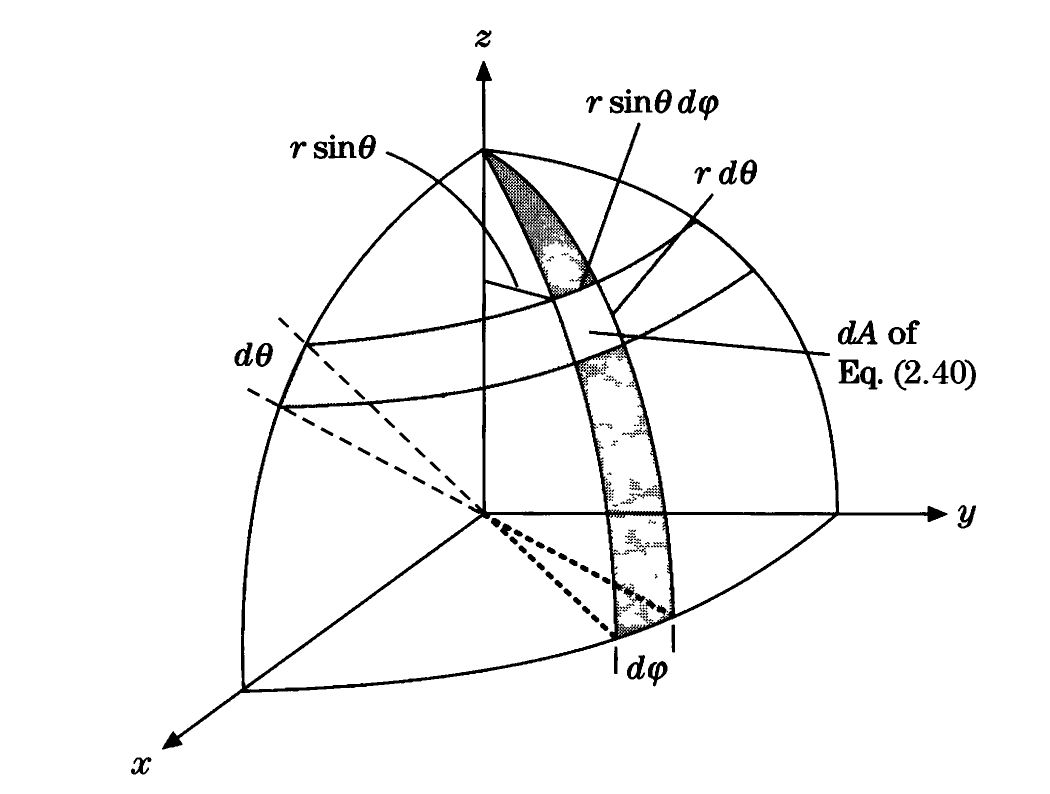
\includegraphics[scale=0.35]{Imagenes/Elemento_Area_Esferico}
    \caption{Elemento de área en el sistema coordenado esférico.}
    \label{fig:figura_elemento_area_esferico}
\end{figure}
Diferenciando las expresiones inversas, tenemos que 
\begin{align}
\begin{aligned}
h_{1} &= h_{r} = 1 \\
h_{2} &= h_{\theta} = r \\
h_{3} &= h_{\varphi} = r \, \sin \theta 
\end{aligned}
\label{eq:ecuacion_02_039}
\end{align}
Lo que nos da un elemento de línea
\[ d \mathbf{r} = \mathbf{\widehat{r}} dr + \bm{\widehat{\theta}} r d\theta + \bm{\widehat{\varphi}} r \sin \theta d \varphi \]
por tanto
\[ ds^{2} = d \mathbf{r} \cdot d \mathbf{r} =  dr^{2} + r^{2} d \theta^{2} + r^{2} \sin^{2} \theta d \varphi^{2} \]
En este sistema coordenado esférico, el elemento de área (para $r=\text{constante}$) es:
\[ dA = d\sigma_{\theta \varphi} = r^{2} \sin \theta d\theta d\varphi \]
Integrando sobre la coordenada azimutal $\varphi$, se tiene que el elemento de área, genera un anillo de ancho $d\theta$
\[ dA_{\theta} = 2 \pi r^{2} \sin \theta d \theta \]
Esta expresión se presenta frecuentemente en problemas con coordenadas esféricas polares con simetría azimutal, tales como la dispersión de un haz no polarizado de partículas nucleares.
\\
Por definición de estereoradianes, un elemento de ángulo sólido $d\Omega$ está dado por:
\[ d \Omega = \dfrac{dA}{r^{2}} = \sin \theta d \theta d \varphi \]
Integrando sobre toda la superficie esférica, se obtiene
\[ \int d \Omega = 4 \pi \]
El elemento de volumen es:
\begin{eqnarray}
\begin{aligned}
d \tau &= r^{2} dr \sin \theta d \theta d\varphi \\
&= r^{2} d r d \Omega
\end{aligned}
\end{eqnarray}
Los vectores unitarios del sistema polar esféricos se muestran en la siguiente figura:
%\begin{figure}[!h]
%\centering
%\tdplotsetmaincoords{60}{110}
%%
%\pgfmathsetmacro{\rvec}{.8}
%\pgfmathsetmacro{\thetavec}{30}
%\pgfmathsetmacro{\phivec}{60}
%%
%\begin{tikzpicture}[scale=5,tdplot_main_coords]
%    \coordinate (O) at (0,0,0);
%    \draw[thick,->] (0,0,0) -- (1,0,0) node[anchor=north east]{$x$};
%    \draw[thick,->] (0,0,0) -- (0,1,0) node[anchor=north west]{$y$};
%	\draw[thick,->] (0,0,0) -- (0,0,1) node[anchor=south]{$z$};
%    \tdplotsetcoord{P}{\rvec}{\thetavec}{\phivec}
%    \draw[-stealth,color=red] (O) -- (P) node[above right] {$P$};
%    \draw[dashed, color=red] (O) -- (Pxy);
%    \draw[dashed, color=red] (P) -- (Pxy);
%    %\draw[dashed, color=red] (0,0,0.7) -- (O);
%    \tdplotdrawarc{(O)}{0.4}{0}{\phivec}{anchor=north}{$\phi$}
%    \tdplotsetthetaplanecoords{\phivec}
%    \tdplotdrawarc[tdplot_rotated_coords]{(0,0,0)}{0.5}{0}%
%        {\thetavec}{anchor=south west}{$\theta$}
%
%
%\end{tikzpicture}
%\end{figure}
Se insiste en que los vectores unitarios $\mathbf{\widehat{r}}, \bm{\widehat{\theta}}, \bm{\widehat{\varphi}}$ cambian de dirección conforme cambian los ángulos $\theta$ y $\varphi$. En términos de los vectores unitarios cartesianos $(\mathbf{i},\mathbf{j},\mathbf{k})$ cuya dirección es fija, tenemos que
\begin{eqnarray}
\begin{aligned}
\mathbf{\widehat{r}} &= \mathbf{\widehat{x}}\sin \theta \cos \varphi + \mathbf{\widehat{y}} \sin \theta \sin \varphi + \mathbf{\widehat{z}} \cos \theta \\
\bm{\widehat{\theta}} &= \mathbf{\widehat{x}}\cos \theta \cos \varphi + \mathbf{\widehat{y}} \cos \theta \sin \varphi - \mathbf{\widehat{z}} \sin \theta = \dfrac{\partial \mathbf{\widehat{r}}}{\partial \theta} \\
\bm{\widehat{\varphi}} &= - \mathbf{\widehat{x}} \sin \varphi + \mathbf{\widehat{y}} \cos \varphi = \dfrac{1}{\sin \theta} \dfrac{\partial \mathbf{\widehat{r}}}{\partial \varphi}
\end{aligned}
\end{eqnarray}
Dadas la transformación inversa y un vector dado, se puede expresar de diferentes maneras, por ejemplo el vector de posición $\mathbf{r}$ puede escribirse como
\[ \begin{split}
\mathbf{r} &= \mathbf{\widehat{r}} r = \mathbf{\widehat{r}} \left( x^{2} + y^{2} + z^{2} \right)^{1/2} \\
&= \mathbf{\widehat{x}} x + \mathbf{\widehat{y}} y + \mathbf{\widehat{z}} z  \\
&= \mathbf{\widehat{x}} r \sin \theta \cos \varphi + \mathbf{\widehat{y}} r \sin \theta \sin \varphi + \mathbf{\widehat{z}} r \cos \theta    
\end{split}\]
De  acuerdo al problema a resolver, debemos de elegir la expresión más útil.
\\
Renombrando los vectores unitarios del sistema de coordenadas curvilineas $(\mathbf{q}_{1}, \mathbf{q}_{2}, \mathbf{q}_{3}) $ como $(\mathbf{\widehat{r}}, \bm{\widehat{\theta}}, \bm{\widehat{\varphi}})$, los operadores diferenciales son:
\begin{eqnarray}
\nabla \psi &=& \mathbf{\widehat{r}} \dfrac{\partial \psi}{\partial r} + \bm{\widehat{\theta}} \dfrac{1}{r} \dfrac{\partial \psi}{\partial \theta} + \bm{\widehat{\varphi}} \dfrac{1}{r \sin \theta} \dfrac{\partial \psi}{\partial \varphi} \\
\mathbf{\nabla \cdot V} &=& \dfrac{1}{r^{2} \sin \theta} \left[ \sin \theta \dfrac{\partial}{\partial r}(r^{2} V_{r}) + r \dfrac{\partial}{\partial \theta} (\sin \theta V_{\theta}) + r \dfrac{\partial V_{\varphi}}{\partial \varphi} \right] \\
\mathbf{\nabla \cdot \nabla \psi} &=& \dfrac{1}{r^{2} \sin \theta} \left[  \sin \theta \dfrac{\partial}{\partial r} \left(  r^{2} \dfrac{\partial \psi}{\partial r} \right) + \dfrac{\partial}{\partial \theta} \left( \sin \theta \dfrac{\partial \psi}{\partial \theta} \right) + \dfrac{1}{\sin \theta} \dfrac{\partial^{2} \psi}{\partial \varphi^{2}}   \right] \\
\mathbf{\nabla \times V} &=& \dfrac{1}{r^{2} \sin \theta}
\renewcommand\arraystretch{1.5} \begin{vmatrix}
\mathbf{\widehat{r}} & r \bm{\widehat{\theta}} & r \sin \theta \bm{\widehat{\varphi}} \\
\dfrac{\partial}{\partial r} & \dfrac{\partial}{\partial \theta} & \dfrac{\partial}{\partial \varphi} \\
V_{r} & r V_{\theta} & r \sin \theta V_{\varphi}
\end{vmatrix}
\end{eqnarray}
\section{Construcción de sistemas coordenados.}
Para construir un sistema de coordenadas en un espacio euclidiano basta contar con una familia de curvas planas, definida en forma tal que a cada valor de un parámetro le corresponda una curva. La teoría vista nos permite construir una familia de curvas ortogonales a la familia original. De este modo se obtiene un sistema de coordenadas curvilíneas ortogonales en el plano. Por rotación o adición del eje $z$ pueden generarse sistemas coordenados en 3D. Así, las coordenadas cilíndricas y esféricas pueden ser obtenidas de las coordenadas polares incluyendo el eje $z$ o rotando alrededor del eje $y$.
\subsection*{Coordenadas parabólicas cilíndricas.}
La ecuación de la familia de parábolas confocales, cuyo foco coincide con el origen de coordenadas tiene la forma:
\begin{equation}
y^{2} = 4 \: p \: (p + x)
\label{eq:ecuacion_cpc_01_50}
\end{equation}
La cúspide de estas parábolas apunta a la izquierda. Para cada valor de $p: 0 \to \infty$, hay una parábola. El conjunto de parábolas con diferente valor de $p$ pero el mismo foco es \emph{confocal}. Si escribimos
\[ f(x,y) = y^{2} - 4 \: p \: (p + x) \]
se tiene que el gradiente es
\begin{equation}
\nabla f = - 4 \: p \: \mathbf{\widehat{e}_{x}} + 2 \: y  \mathbf{\widehat{e}_{y}}
\nabla f = - 4 \: p \: \mathbf{\widehat{e}_{x}} + 2 \: y  \mathbf{\widehat{e}_{y}}
\label{eq:ecuacion_cpc_01_51}
\end{equation}
es un vector perpendicular a la curva (\ref{eq:ecuacion_cpc_01_50}), para un valor específico de $p$.
\par
Con el fin de que $\nabla f$ sea perpendicular a \emph{todas} las parábolas debemos de eliminar $p$ de la ec. (\ref{eq:ecuacion_cpc_01_51}), usando la ec. (\ref{eq:ecuacion_cpc_01_50}). 

Se sigue que: $2 \: p = -x + \sqrt{x^{2} + y^{2}}$ para $p \geq 0$, por lo que
\[  \nabla f =  -2 \left( -x + \sqrt{x^{2} + y^{2}} \right) \: \mathbf{\widehat{e}_{x}} + 2 \: y \: \mathbf{\widehat{e}_{y}} \]
La ecuación de las curvas ortogonales a la familia de parábolas es $\nabla f \times d \mathbf{r} = 0$ de donde sigue con $d \mathbf{r} = \mathbf{\widehat{e}_{x}} \: dx + \mathbf{\widehat{e}_{y}}\:  dy$:
\[ y \: dx +  \left( - x + \sqrt{x^{2} + y^{2}} \right) \: dy = 0 \]
si hacemos $y = v \: x$, tendremos
\[ \dfrac{dv}{v} \left[ 1 - \dfrac{1}{\sqrt{1 + v^{2}}} \right] + \dfrac{dx}{x} = 0 \]
de donde
\begin{equation}
 y^{2} = 4 \: c (c - x)
 \label{eq:ecuacion_cpc_01_52}
\end{equation}
Esta es otra familia de parábolas confocales cuya cúspide apunta a la derecha. Usaremos $c \geq 0$.
\par
Con las familias (\ref{eq:ecuacion_cpc_01_50}) y (\ref{eq:ecuacion_cpc_01_52}) definimos las coordenadas parabólicas.
\\
Para cada pareja $(p, c)$ hay un pareja de parábolas ortogonales que se cruzan en un punto al que llamaremos $(p, c)$, correspondiente a $(x, y)$.
\par
Por definición las coordenadas parabólicas planas $(\eta, \xi)$ son:
\[ 2 \: p = \eta^{2} \hspace{1cm} 2 \: c = \xi^{2} \]
La regla de transformación entre coordenadas cartesianas y parábolicas planas, tiene entonces la forma:
\[ x = \dfrac{\xi^{2} - \eta^{2}}{2} \hspace{1cm} y = \eta \: \xi \]
Escogemos $\eta:0 \to \infty$. Con el fin de lograr que $y = \eta \: \xi$ pueda tomar valores negativos hemos de escoger $\xi = -\infty to \infty$.
\par
Definimos las coordenadas \textbf{parabólicas cilíndricas} adicionando la coordenada cartesiana $z$ a las coordenadas parabólicas planas $(\eta, \xi)$. En este caso:
\begin{align*}
\mathbf{r} &= x \: \mathbf{\widehat{i}} + y \: \mathbf{\widehat{j}} + \mathbf{\widehat{k}} \\
&= \dfrac{\mathbf{\widehat{i}}}{2} \left( \xi^{2} - \eta^{2} \right) + \eta \: \xi \: \mathbf{\widehat{j}} + z \: \mathbf{\widehat{k}}
\end{align*}
Por lo que los factores de escala son
\[ h_{\xi} = h_{\eta} = \sqrt{\xi^{2} + \eta^{2}}, \hspace{0.5cm} h_{z} = 1  \]
Si en vez de adicionar la coordenada $z$ realizamos una rotación de las coordenadas parabólicas planas alrededor del eje $x$ obtendremos, en vez de $y$, dos nuevos ejes $y$, y $z$ y una nueva coordenada $\varphi$, tal que: $y = \eta \: \xi \: \cos \varphi$ y $z= \eta \: \xi \: \sin \varphi$.
\par
Esta rotación da lugar a dos familias de paraboloides de revolución que originan un sistema de coordenadas parabólicas.
\\
En este caso, y después de reemplazar $x \to z$; $y \to x$; $z to y$ podemos escribir:
\[ x = \eta \: \xi \: \cos \varphi, \hspace{0.5cm} y = \eta \: \xi \: \sin \varphi, \hspace{0.5cm} z = \dfrac{\xi^{2} -\eta^{2}}{2} \]
con $0 \leq \xi < \infty$, $0 \leq \eta < \infty$, $0 \leq \varphi \leq 2 \pi$. Es fácil demostrar que
\[ h_{\xi} = h_{\eta} = \sqrt{\xi^{2} + \eta^{2}}, \hspace{0.5cm} h_{\varphi} = \eta \: \xi  \]
Las superficies coordenadas de este sistema son: dos familias de paraboloides de revolución alrededor del eje $z$ correspondientes a $\xi = \mbox{ constante}$ y $\eta = \mbox{ constante}$, y planos meridianos $\varphi = \mbox{ constante}$.
\\
El siguiente paso es calcular en coordenadas parabólicas.
\begin{enumerate}
\item $\nabla \varphi$.
\item $\nabla \cdot A$.
\item $\nabla \times A$.
\item $\nabla^{2} \varphi$.
\end{enumerate}
\subsection*{Coordenadas cilíndricas esféricas $(u, \theta, z)$}
Están dadas por:
\begin{eqnarray}
\begin{aligned}
x &= a \cosh u \cos \theta \\
y &= a \sinh u \sin \theta \\
z &= z
\end{aligned}
\end{eqnarray}
donde $a$ es una constante.
\subsection*{Coordenadas toroidales $(\xi,\chi,\varphi)$}
Están definidas por las ecuaciones de transformación:
\begin{eqnarray}
\begin{aligned}
x &=& \dfrac{a \sinh \xi \cos \varphi}{\cosh \xi - \cos \chi} \\
y &=& \dfrac{a \sin  \xi \sin \varphi}{\cosh \xi - \cos \chi} \\
z &=& \dfrac{a \sin \chi}{\cosh \xi - \cos \chi}
\end{aligned}
\end{eqnarray}
\end{document}